\documentclass[12pt]{article}
\usepackage[utf8]{inputenc}
\usepackage{lmodern} % Ensures all font shapes are available
\usepackage{graphicx}
\usepackage{hyperref}
\usepackage{minted}
\usepackage{float}
\usepackage{geometry}
\geometry{margin=1in}


\title{Moneyworth Web App Project Report}
\author{Kazibwe David Nelson (2400724054) \and Sseruwagi Don Marvin (2400724775) \and Mila Samantha Likiya (2400724201) \and Mayanja Joel Stephen (2400724184)}
\date{May 15, 2025}

\begin{document}
\maketitle

\section{Problem Statement}
Sales managers struggle to create, organize, and follow sales records through traditional or ad-hoc products, which creates unstructured data, reduced efficiency, and lost opportunities. A contemporary, Web-based system, which can make these operations easy within a Web 2.0 environment, is required. Present systems are generally devoid of integrated authentication, inherent selling reporting, and interactive plotting, and follow double verification schemes. Moneyworth is presented for filling the gaps.It has the following pages:

\subsection{Home}
The Home page features a welcoming jumbotron section with summary cards. Each card includes a call-to-action button linking to either the ``Create Sale'' or ``Browse Sales'' page. This design helps users quickly access the main functions of the app.
\begin{figure}[H]
    \centering
    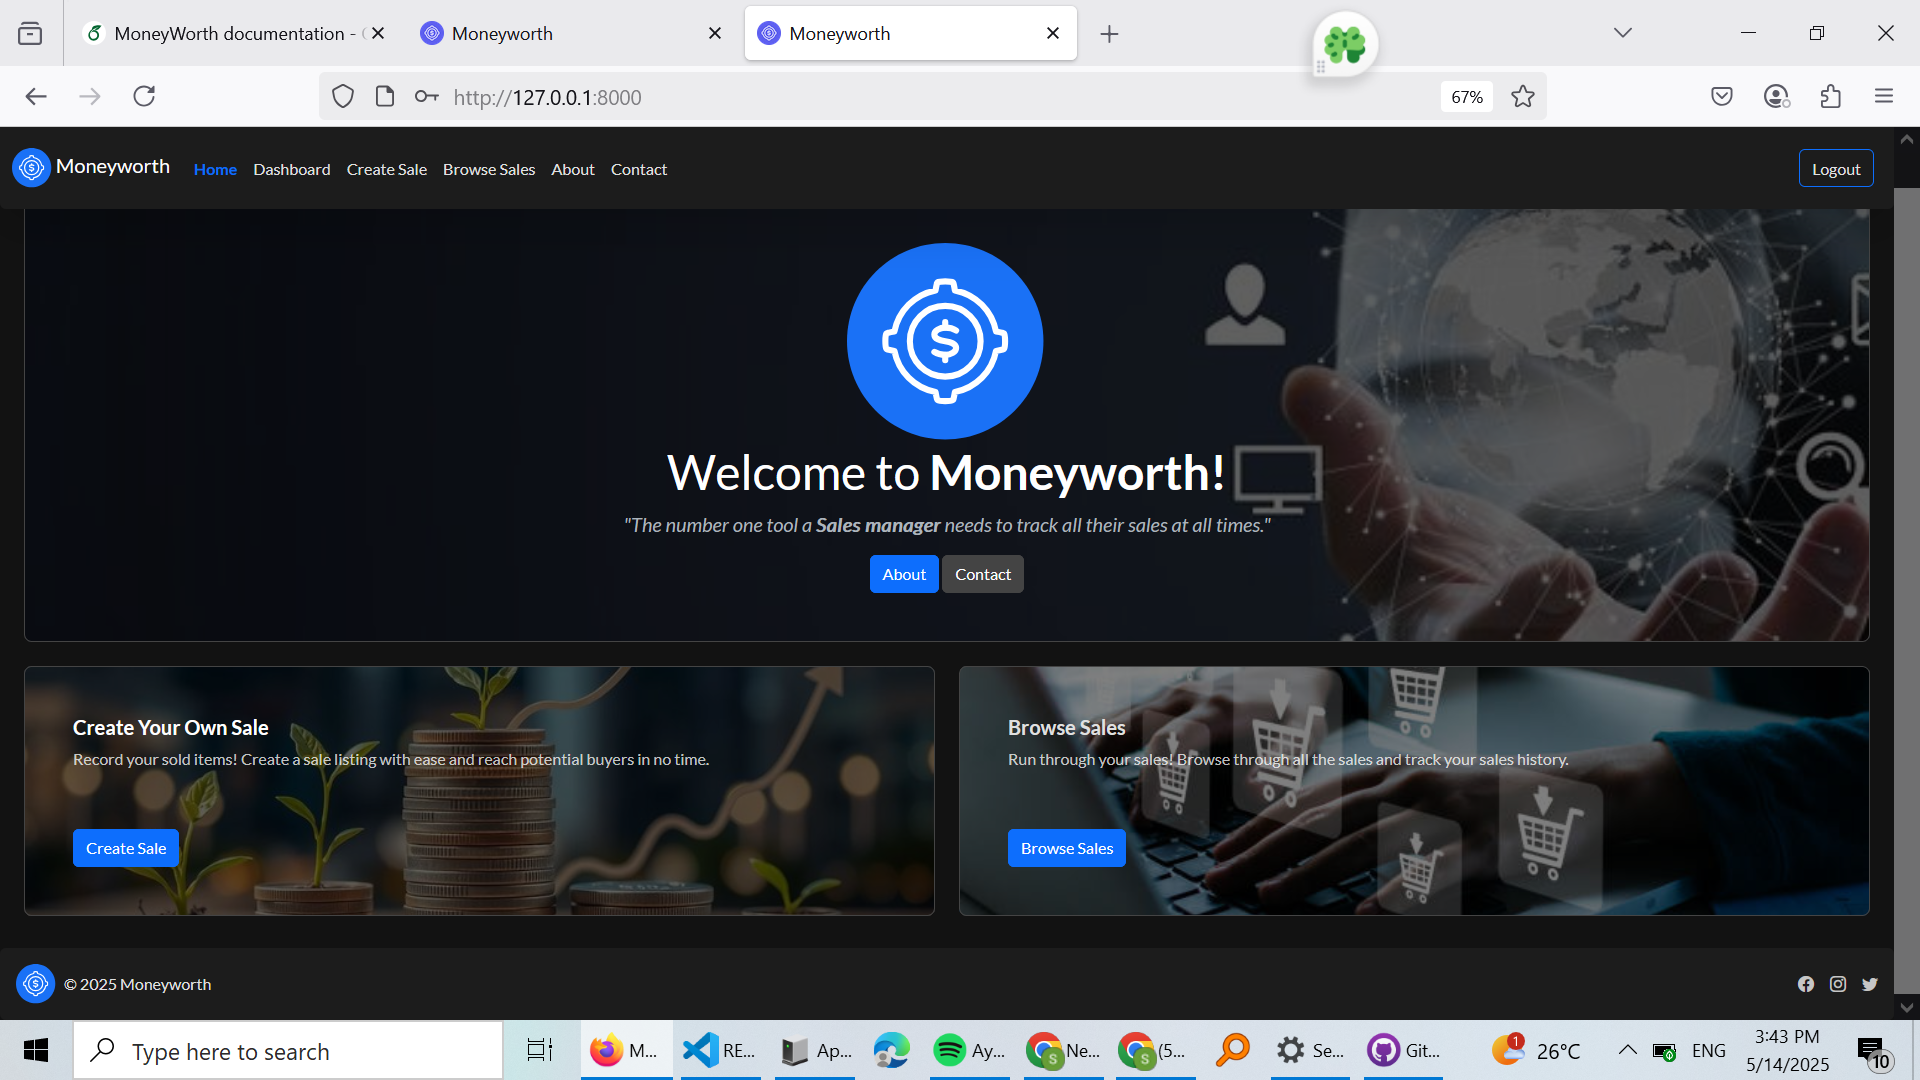
\includegraphics[width=0.5\textwidth]{home.png}
    \caption{The Home page of the application, featuring navigation and summary cards.}
\end{figure}

\subsection{Dashboard}
The Dashboard page displays summary cards that provide an overview of sales performance:
\begin{itemize}
    \item \textbf{Total sales:} The total number of sales recorded in the system.
    \item \textbf{Active sales:} The number of sales that are fully paid and currently in progress.
    \item \textbf{Pending sales:} The number of sales with partial payments.
    \item \textbf{Completed sales:} The number of sales that are fully paid and completed.
\end{itemize}
The Dashboard also includes a table of recent sales and call-to-action (CTA) buttons that link to the ``Create Sale'' and ``Browse Sales'' pages for quick access.
\begin{figure}[H]
    \centering
    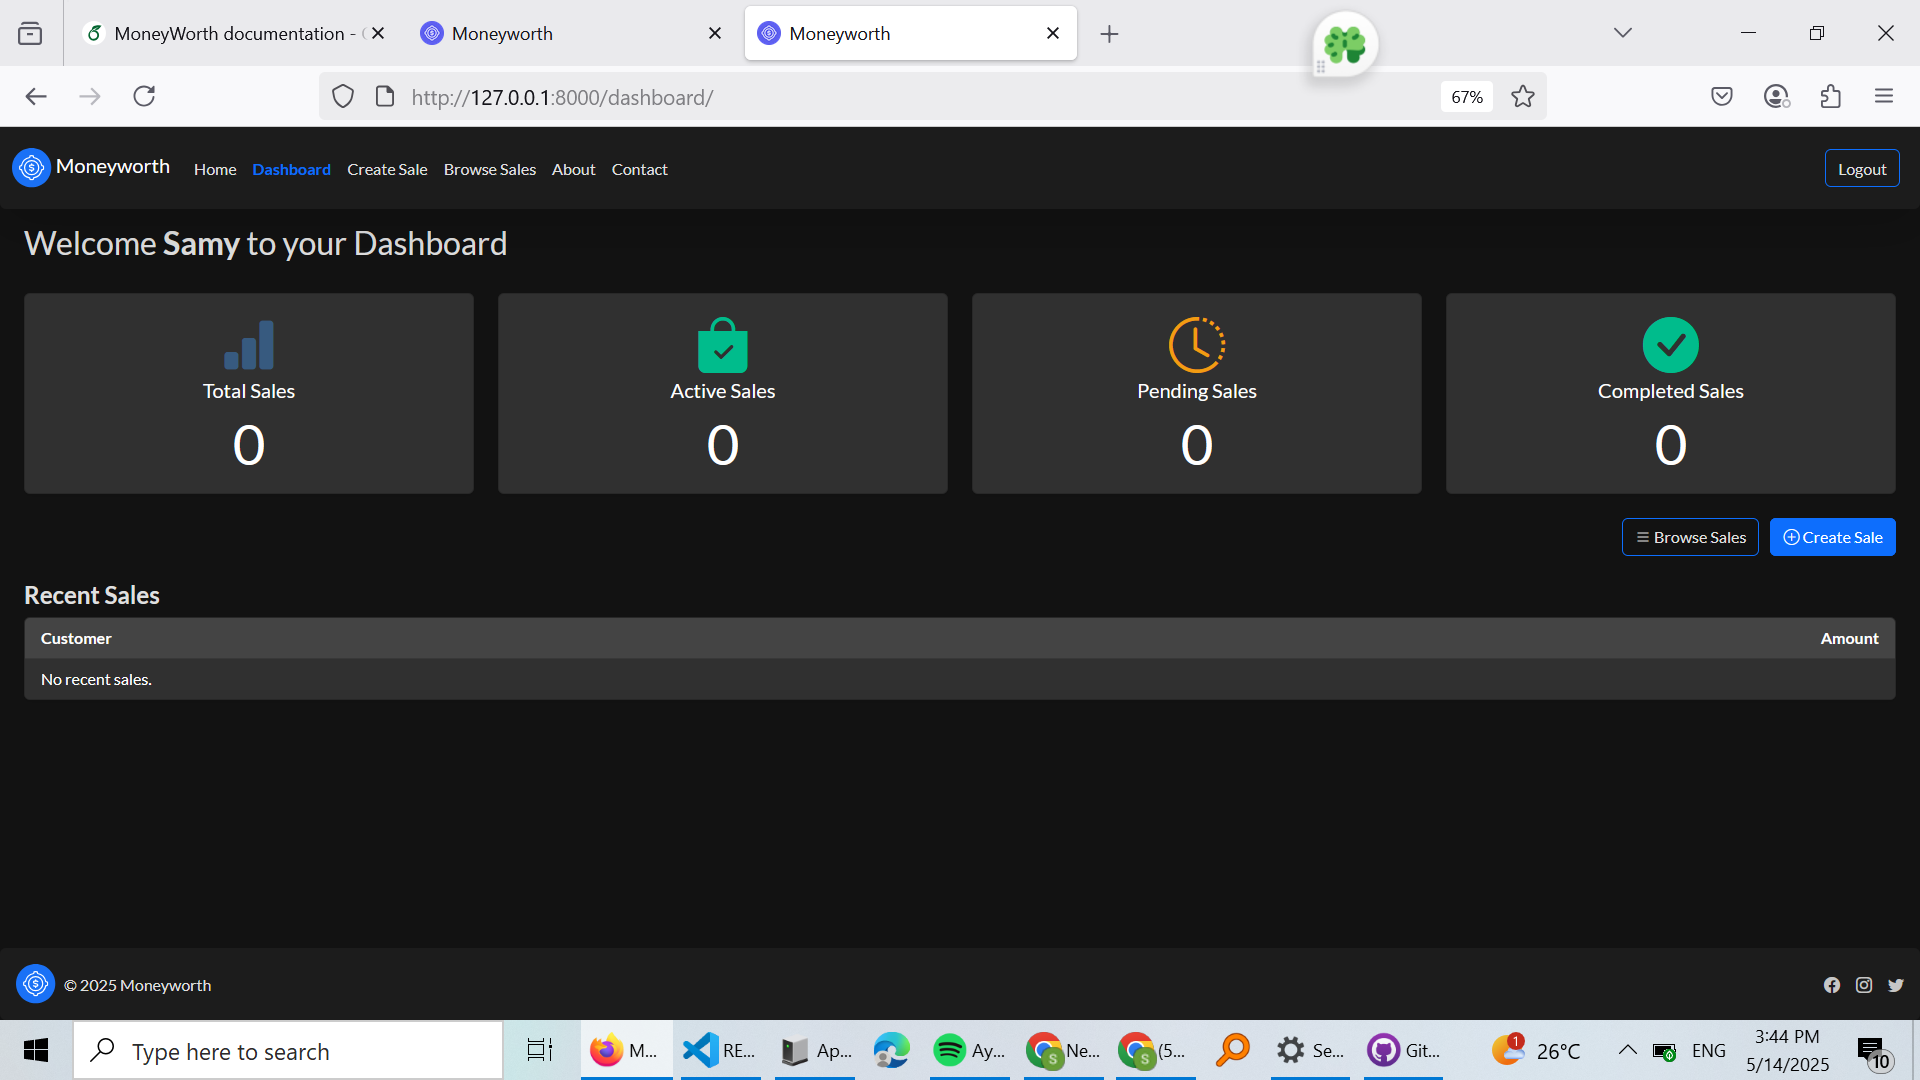
\includegraphics[width=0.5\textwidth]{dashboard.png}
    \caption{The Dashboard page displaying user statistics and performance charts.}
\end{figure}

\subsection{Browse Sales}
The Browse Sales page presents a table of all sales records, each identified by a unique ID. It also provides a search bar for filtering results and a CTA button that directs the user to the Create Sale page. This page allows users to quickly find and review existing sales entries.
\begin{figure}[H]
    \centering
    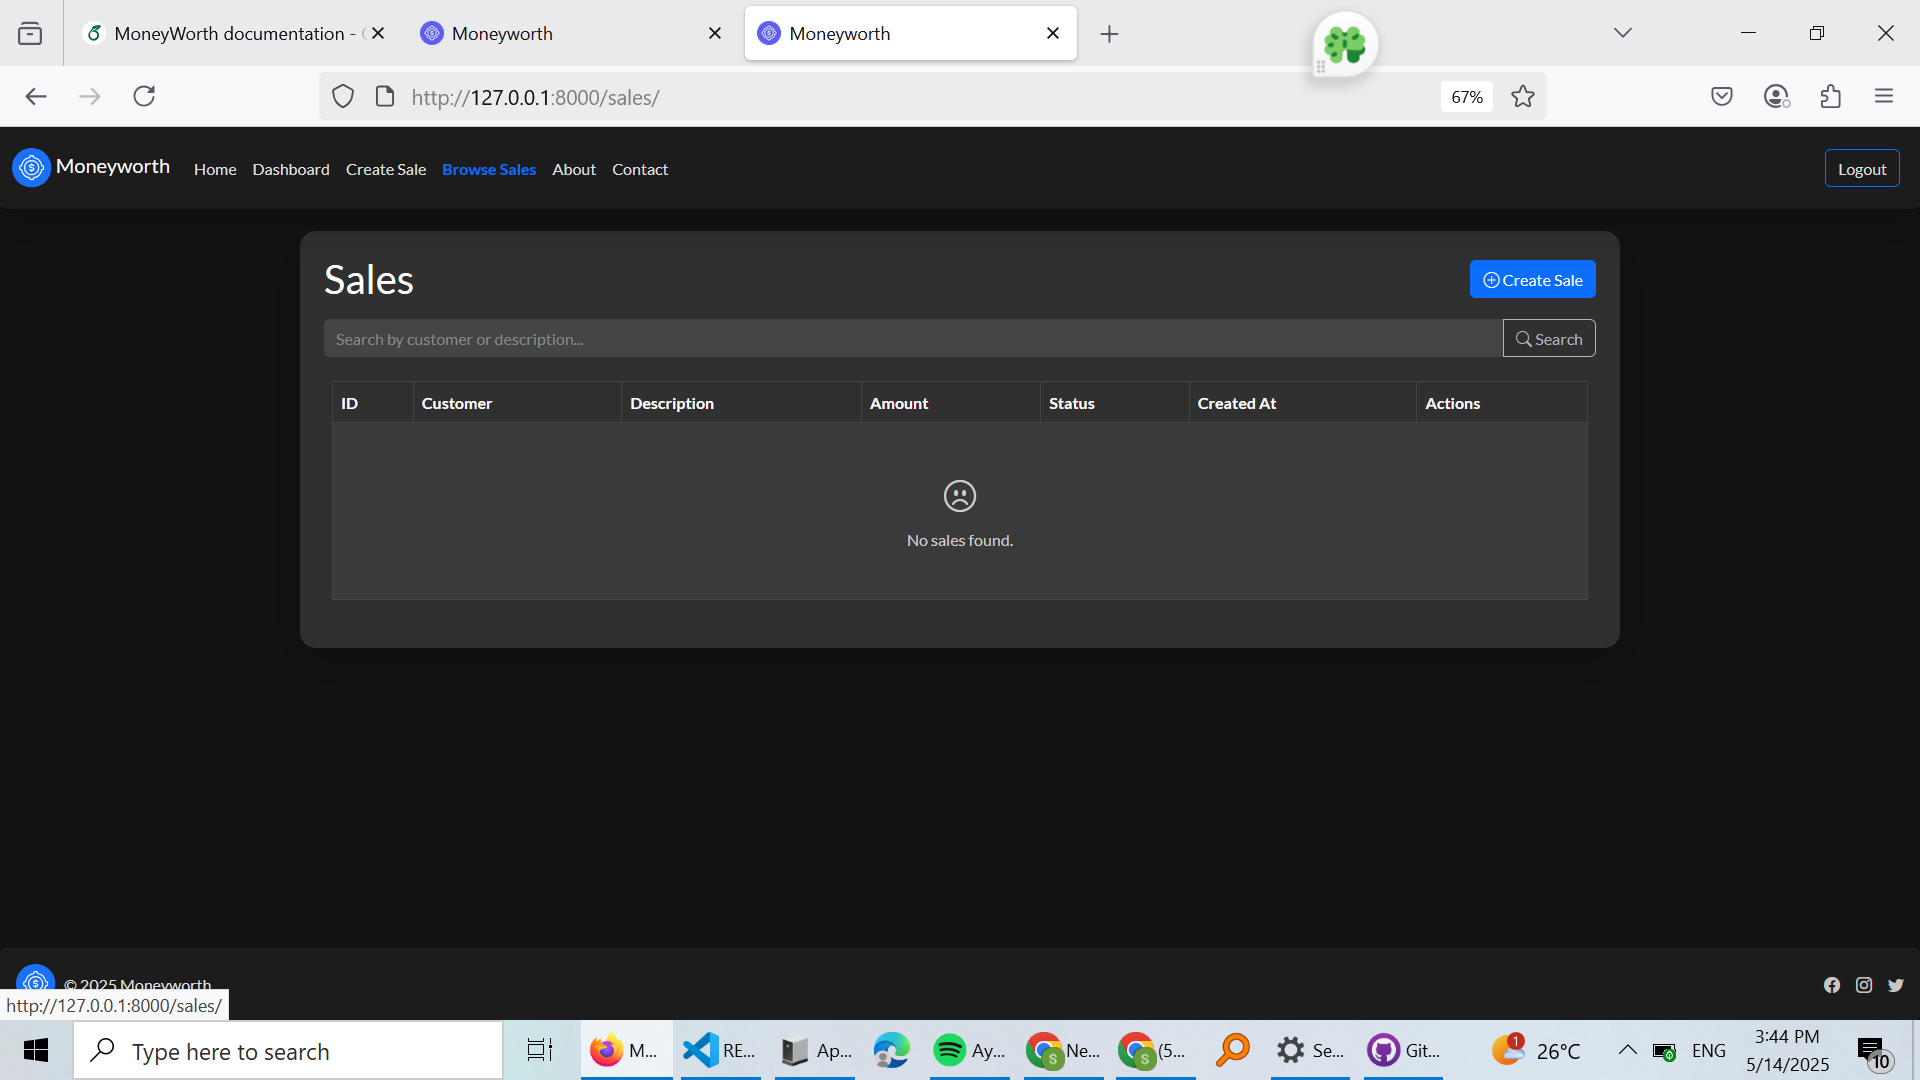
\includegraphics[width=0.5\textwidth]{browse_sales.png}
    \caption{The Browse Sales page showing a table of all sales records.}
\end{figure}

\subsection{Create Sale}
The Create Sale page contains a form with fields for entering details of a new sale, such as the product name, quantity, and price. This page enables users to add new sales records to the system.
\begin{figure}[H]
    \centering
    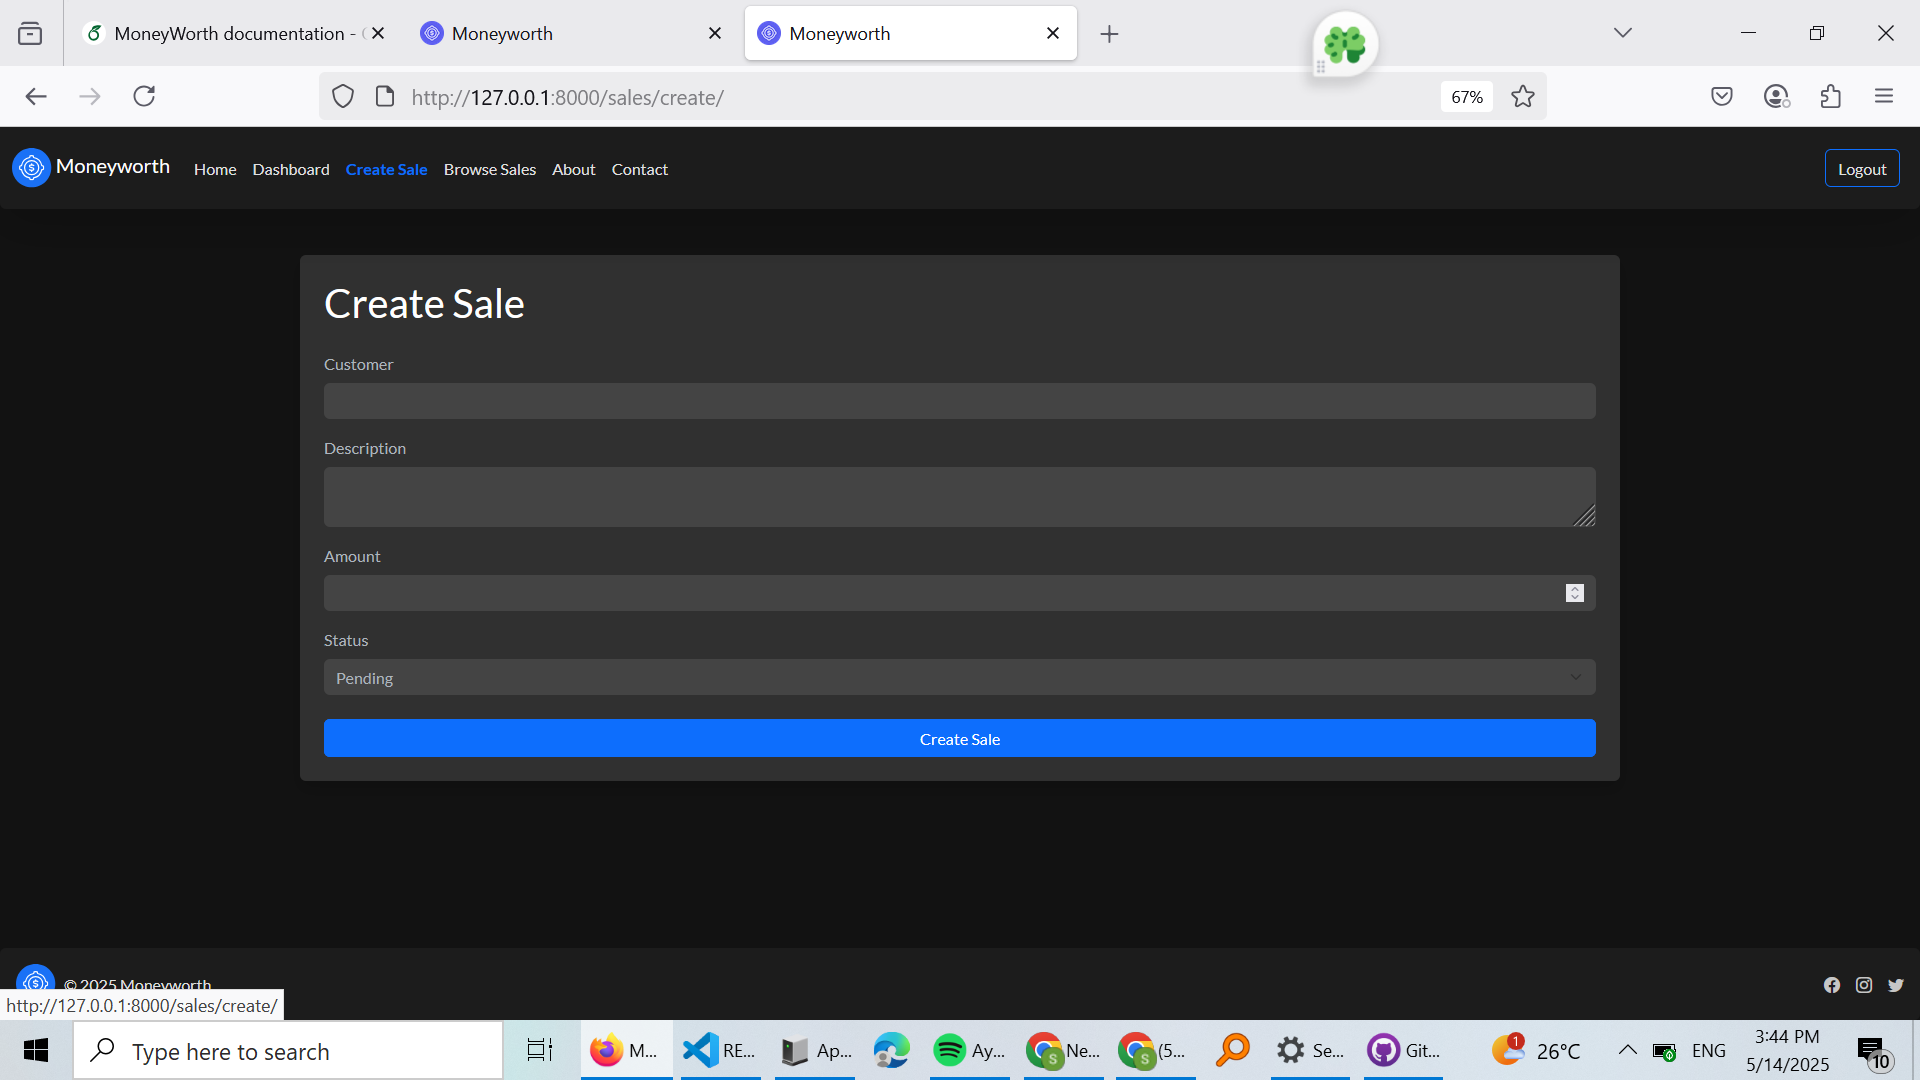
\includegraphics[width=0.5\textwidth]{create_sales.png}
    \caption{The Create Sale page with a form for adding a new sales record.}
\end{figure}

\subsection{About}
The About page provides a brief introduction to the Moneyworth sales app. It highlights the team behind the development of the application and the vision and mission of the project.
\begin{figure}[H]
    \centering
    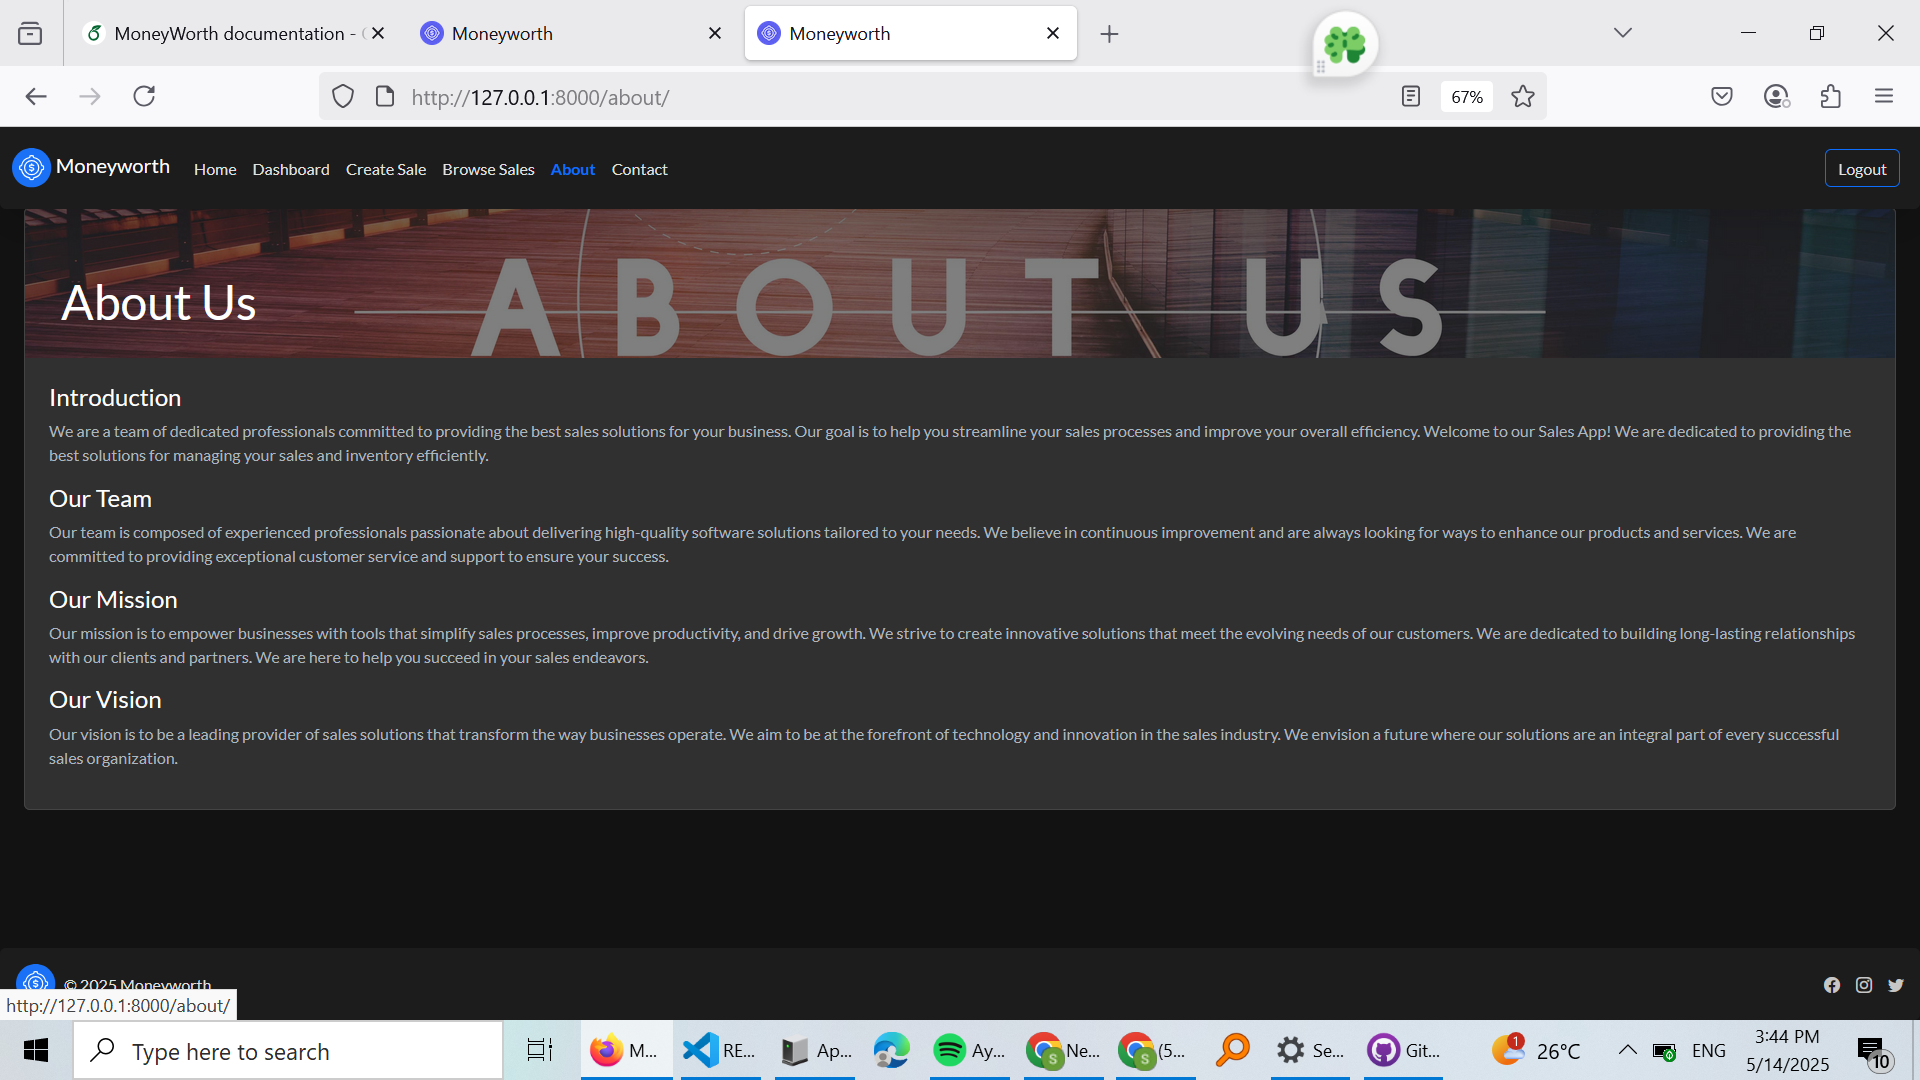
\includegraphics[width=0.5\textwidth]{about_us.png}
    \caption{The About page of the application, describing its purpose and development team.}
\end{figure}

\subsection{Contact}
The Contact page provides users with a form to reach out to the development team or support staff. It includes fields for the user's name, email, and message, facilitating communication between users and developers.
\begin{figure}[H]
    \centering
    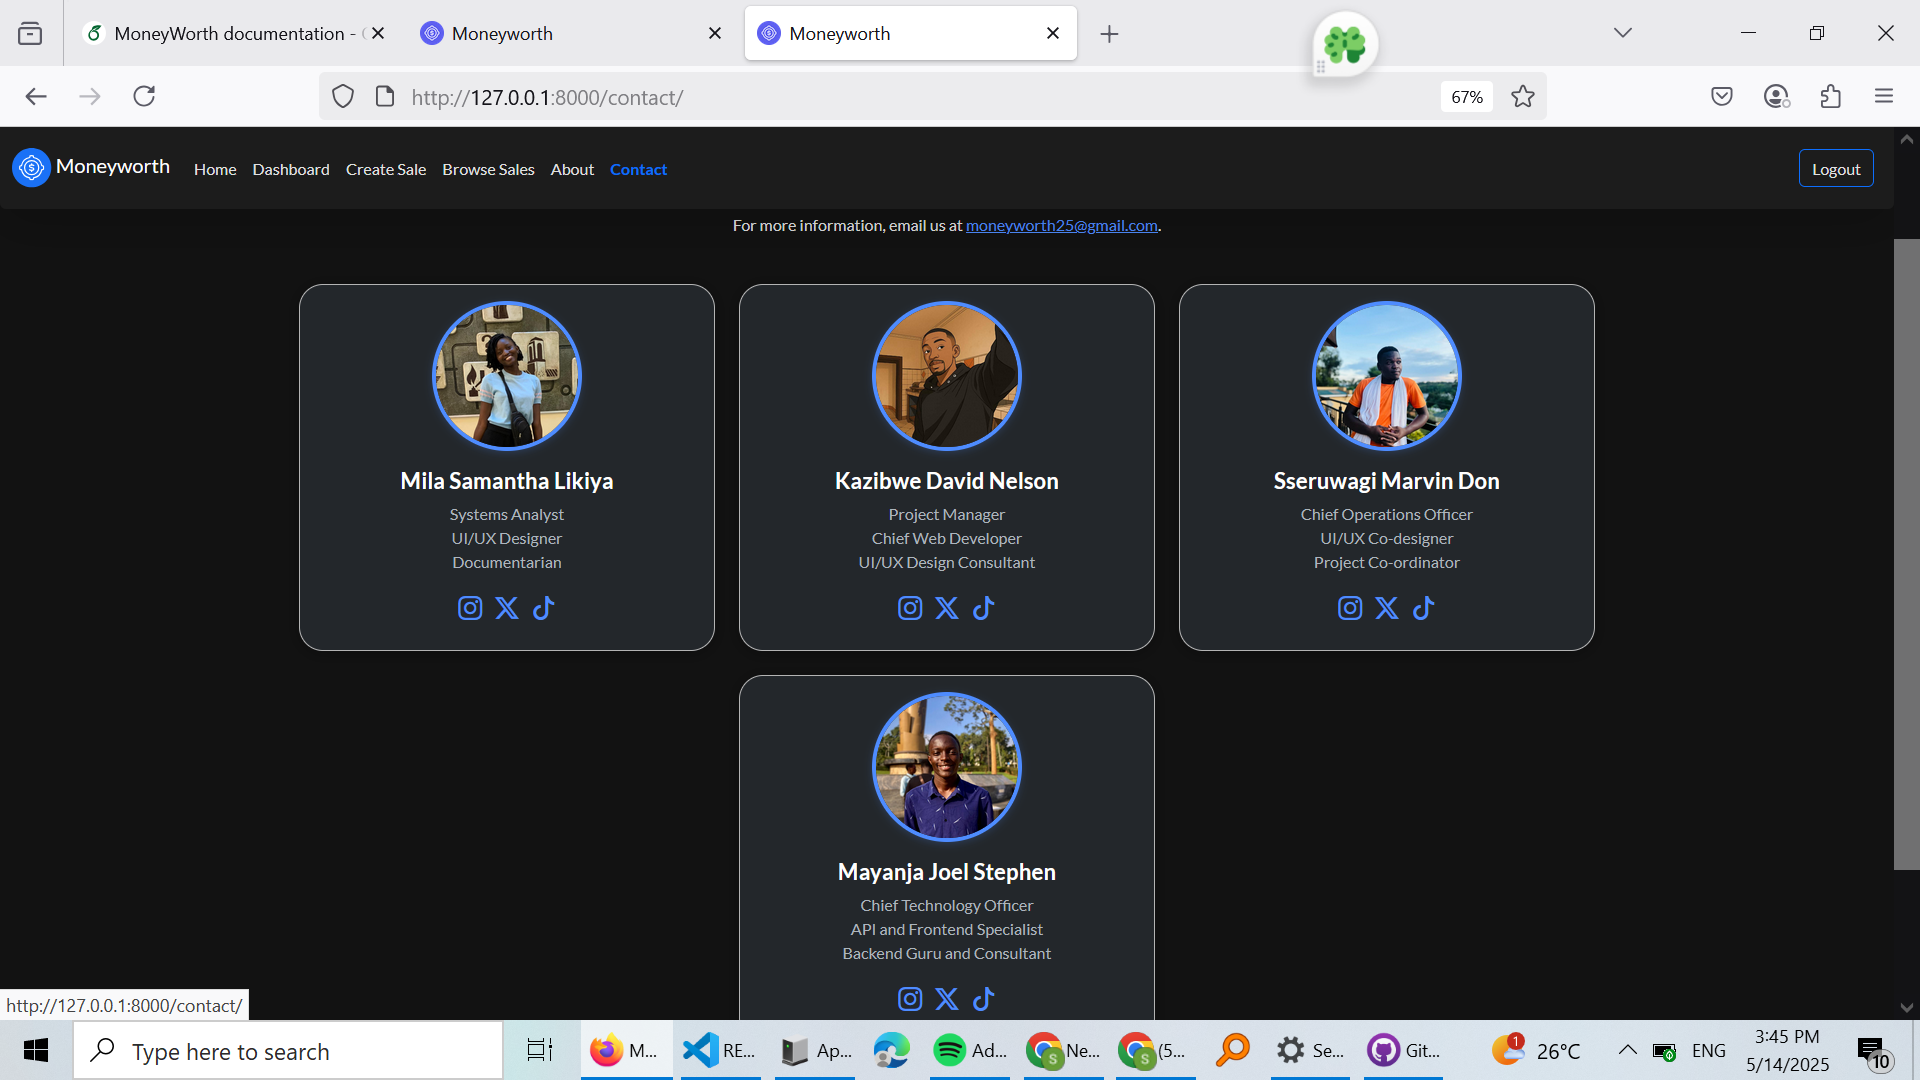
\includegraphics[width=0.5\textwidth]{contact_us.png}
    \caption{The Contact page offering a form to contact the development team.}
\end{figure}

\section{HTML and Django Template Code Implementation}
This section presents the HTML and Django template code used to implement the project's layout.

\subsection{Base Template Explanation}
The base template, \texttt{base.html}, defines the overall structure of the site. It includes a navigation bar, a hero (jumbotron) section on the Home page, and a footer. Content blocks are defined using Django's template tags, allowing child templates to override specific sections. For example:

\begin{minted}[fontsize=\small]{html}

<!DOCTYPE html>
<html lang="en">
<head>
    <meta charset="UTF-8">
    <title>Django Sales App</title>
    <link rel="stylesheet" href="">
    <link rel="stylesheet" href="">
    
</head>
<body>
    <nav>...navbar code...</nav>
    
    <footer>...footer code...</footer>
    <script src=""></script>
</body>
</html>
\end{minted}

\subsection{Child Template Example}
A child template (for instance, \texttt{home.html}) extends the base template and fills in the designated content blocks:

\begin{minted}[fontsize=\small]{html}


Home - Django Sales App


<div class="jumbotron">
    <h1>Welcome to the Django Sales App!</h1>
    <p>Browse and manage sales listings easily.</p>
</div>

\end{minted}

\subsection{Use of Template Tags}
Key Django template tags used in this project include:
\begin{itemize}
    \item \verb||: Allows a template to inherit from a base template.
    \item \verb||: Defines sections of content that child templates can override.
    \item \verb||: Resolves the URL for static files (CSS, JavaScript, images).
\end{itemize}
These tags help organize the templates, promote code reuse, and simplify static file management.

\subsection{URL and View Structure}
The \texttt{urls.py} and \texttt{views.py} files connect URLs to view functions and templates. For example:

\begin{minted}[fontsize=\small]{python}
# core/urls.py
from django.urls import path
from . import views

urlpatterns = [
    path('', views.home, name='home'),
    path('dashboard/', views.dashboard, name='dashboard'),
    path('sales/', views.browse_sales, name='browse_sales'),
    path('sales/create/', views.create_sale, name='create_sale'),
    path('about/', views.about, name='about'),
    path('contact/', views.contact, name='contact'),
]
\end{minted}

\begin{minted}[fontsize=\small]{python}
# core/views.py
from django.shortcuts import render

def home(request):
    return render(request, 'core/home.html')

# ...other view functions...
\end{minted}

\section{Benefits of Django for Responsive Web Apps}
Django is ideal for responsive web apps due to its clear separation of logic and presentation (MTV architecture), easy integration with Bootstrap for mobile-friendly design, and built-in support for security, scalability, and fast development.

\section{Linking Static CSS and JavaScript in Django}
To include static files (CSS and JavaScript) in Django:
\begin{enumerate}
    \item Set \texttt{STATIC\_URL} in \texttt{settings.py} (e.g., \texttt{STATIC\_URL = '/static/'}).
    \item Add \verb|| at the top of each template.
    \item Reference static files using \verb|| (for example, \verb||).
\end{enumerate}
For example:

\begin{minted}[fontsize=\small]{html}

<link rel="stylesheet" href="">
\end{minted}

\section{Components of MTV Architecture in Django}
Django follows the Model-Template-View (MTV) architecture:
\begin{itemize}
    \item \textbf{Model:} Defines the data structure. For example, the \texttt{Sales} model in \texttt{core/models.py} manages the sales data.
    \item \textbf{View:} Handles requests and returns responses. In this project, functions in \texttt{core/views.py} render templates for each page based on the request.
    \item \textbf{Template:} Renders the HTML presentation. Template files (e.g., in \texttt{templates/core/}) define what the user sees in the browser.
\end{itemize}

\end{document}
